\documentclass[12pt, letterpaper]{article}
\usepackage[utf8]{inputenc}
\usepackage[english]{babel}
\usepackage[left=0.5in,top=0.5in,bottom=1in,right=0.5in]{geometry}
\usepackage{amsmath, amsthm}
\usepackage{amssymb}
\usepackage{graphicx}
\usepackage{epstopdf}
\usepackage{scrextend}
\usepackage{hyperref}
%\usepackage[document]{ragged2e}

\hypersetup{
	colorlinks=true,
	linkcolor=blue,
	filecolor=magenta,      
	urlcolor=cyan,
	pdftitle={Sharelatex Example},
	bookmarks=true,
	%pdfpagemode=FullScreen,
}

\makeatletter
\renewcommand{\@seccntformat}[1]{\csname the#1\endcsname.\quad}
\makeatother

\makeatletter
%\usepackage{multicol}
%\setlength{\columnsep}{1cm}

\begin{document}
\title{Solutions to selected problems}
\author{Igor}
\maketitle

\pagenumbering{roman}
\tableofcontents

\pagenumbering{arabic}
\newpage
\section{Light bar problem}
\paragraph{Problem 2.7.27 from Savchenko 2008 edition.\\}
A light bar with m1 and m2 masses $(m_1 \neq m_2)$ at the ends placed on the support point (in the middle of  bar). Initially it is held in this position. Then it's released.
What is the force N which acts on a support point at the moment just after system is released?

\begin{figure}[!htbp]
	\centering
	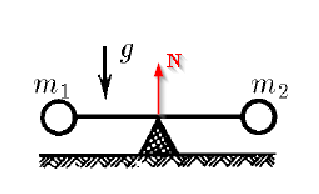
\includegraphics[totalheight=2cm]{./images/LightBarProblem.eps}
	\caption{Light bar problem.}
	\label{fig:verticalcell}
\end{figure}

\noindent\underline{\large Solution:}
\vspace{0.2in}
\begin{addmargin}[1em]{2em}
Moment of inertia:
$$I=(m_1+m_2)r^2$$
Equation of momentum:
$$(m_2-m_1)gr=I\varepsilon=(m2+m1)r^2\varepsilon$$
Force and acceleration $a_c=\varepsilon x$ at the center of mass:
$$F=Ma_c=(m_1+m_2) \cdot a_c$$
Equation of forces acting:
$$F=(m_1+m_2)g-N$$
Assume $m_2>m_1$ and center of mass is at distance $x$ from support point. Then: $$x=\frac {l(m_2-m_1)} {2(m_1+m_2)}$$
Finally: $$N=(m_1+m_2)g-F=...=\frac {4m_1m_2g} {m_1+m_2}$$
\end{addmargin}

\section{Problem 2}
Let's figure it out

\end{document}